\pdfoutput=1
\documentclass[11pt]{article}
\usepackage[margin=0.85in]{geometry}
\usepackage[T1]{fontenc}
\usepackage[utf8]{inputenc}
\usepackage{lmodern}
\usepackage{microtype}
\usepackage{amsmath,amssymb,amsthm}
\usepackage{graphicx}
\usepackage{booktabs}
\usepackage{tabularx}
\usepackage{array}
\usepackage{enumitem}
\usepackage{xurl}
\usepackage[hidelinks]{hyperref}
\usepackage{etoolbox}
\usepackage{caption}
\usepackage{float}
\usepackage{titlesec}
\usepackage{fancyhdr}
\usepackage{lastpage}

\IfFileExists{rs_doi.tex}{% Insert the Research Square DOI only after Research Square assigns it.
% Use the bare DOI, without https://doi.org/ or doi: prefix.
% Example format only: 10.21203/rs.3.rs-1234567/v1
\newcommand{\ResearchSquareDOI}{}
}{\newcommand{\ResearchSquareDOI}{}}
\newcommand{\rsnote}{%
  \ifdefempty{\ResearchSquareDOI}{}{
  \par\smallskip\noindent\textbf{Related preprint record.} A parallel health-informatics preprint is available on Research Square at \href{https://doi.org/\ResearchSquareDOI}{doi:\ResearchSquareDOI}.\par\smallskip}}

\setlength{\parindent}{0pt}
\setlength{\parskip}{0.55em}
\setlist[itemize]{leftmargin=1.5em,itemsep=0.25em,topsep=0.25em}
\renewcommand{\arraystretch}{1.12}
\captionsetup{font=small,labelfont=bf}
\titleformat{\section}{\large\bfseries}{\thesection}{0.6em}{}
\titleformat{\subsection}{\normalsize\bfseries}{\thesubsection}{0.5em}{}
\pagestyle{fancy}
\fancyhf{}
\fancyfoot[C]{\small GLHS systems study -- page \thepage\ of \pageref{LastPage}}
\renewcommand{\headrulewidth}{0pt}

\title{\textbf{GLHS: Task-Bounded Data Minimization and Concurrency Safety for Stateful Longitudinal Healthcare AI}}
\author{Nguyen Ngoc Thien\\
Hai Ba Trung High School, Hue, Vietnam\\
\texttt{kakangocthien109@gmail.com}
\and
Trinh Minh Quang\\
Hai Ba Trung High School, Hue, Vietnam}
\date{August 2026}

\begin{document}
\maketitle

\begin{abstract}
Persistent health AI creates a consistency problem that retrieval quality alone cannot solve. A model may read an authorized view of a longitudinal record, reason over it, and return a persistent proposal only after the record, consent state, authorization, or governing policy has changed. GLHS treats this read-to-write interval as a governance boundary. Its central mechanism is a disclosure-conditioned, co-versioned contract: on the snapshot-bound path, the exact Task-Bounded Health State Snapshot (THSS) actually supplied to the model becomes an auditable dependency of the later persistent proposal, and a Governed State Transition (GST) revalidates the relevant state and governance coordinates before commit. To isolate deterministic clinical invariants from model hallucinations, GLHS employs a Dual-Layer State Barrier: a deterministic non-LLM reconciliation kernel at the gateway handles temporal arithmetic, bitemporal filtering, conflict detection, and Merkle digest validation, while an epistemic clinical arbiter reasons over qualitative nuances. Furthermore, to overcome false-stale aborts in concurrent multi-agent updates across disjoint clinical domains, GLHS introduces Entity-Partitioned DAG Versioning, eliminating false-stale aborts (0.00\% false-stale rate) under disjoint partition workloads. We evaluate the contract through a matched exact-binding causal ablation ($N=320$ logical schedules, 640 executions), PostgreSQL concurrency and service-overhead experiments, governance-writer TOCTOU repetition schedules ($N=12$, 600 runs), bounded finite-state exploration, and model-context studies. In the matched exact-binding ablation, omitting the exact snapshot dependency admitted 256/256 invalid commits, whereas GLHS exact binding rejected all 256/256 invalid attempts while admitting 64/64 valid controls (paired risk difference 1.0, 95\% CI [1.0, 1.0], exact McNemar $p=1.727\times 10^{-77}$). In 600 PostgreSQL TOCTOU repetition runs across 12 logical schedules, zero forbidden commits were observed (10 robust schedules, 2 non-robust classification mismatches). In the 384-subject synthetic cohort, task-bounded minimization reduced prompt token consumption by 87.4\% (mean 412 vs.\ 3,280 tokens, $p < 10^{-40}$) and latency by 68.2\% with a null paired decision delta (70 wins, 73 losses, 241 ties, exact sign test $p=0.867$).
\end{abstract}

\rsnote

\textbf{Keywords:} longitudinal health AI; stateful AI; disclosure-conditioned commit; health-data governance; bitemporal state; snapshot binding; provenance; consent

\section{Introduction}
A longitudinal health record is not simply a collection of documents to retrieve. The same fact can have one clinical effective time and a later knowledge time; sources can disagree; and information that is appropriate for one actor, purpose, or task may be inappropriate for another. A health-AI system can therefore retrieve a relevant item and still present the wrong historical state, disclose more information than the current use requires, or act on context that is no longer valid by the time a proposed change is written back.

The underlying building blocks are well established. Medical database research distinguishes valid time from transaction or knowledge time~\cite{gabrieli1992,kouramajian1994,kumar1998}. In relational database systems, Serializable Snapshot Isolation (SSI) by Cahill et al.~\cite{cahill2008,cahill2009} guarantees data serializability via SIREAD locks by tracking read--write anti-dependencies on underlying data items, but treats external consent/policy changes as application-layer operations. In distributed authorization, systems such as Google Zanzibar (Tang et al.)~\cite{zanzibar2019} guarantee consistent snapshot authorization via Zookies, but decouple access evaluation from physical database transaction writes. Declarative policy engines (e.g., Open Policy Agent~\cite{opa}, AWS Cedar~\cite{cedar}) evaluate consistent snapshot authorization at specified evaluation tokens. FHIR provides Provenance, Consent, and version-aware HTTP primitives~\cite{fhirprov,fhirconsent,fhirhttp}; openEHR maintains versioned and reconstructable EHR contributions~\cite{openehr}; and W3C PROV provides a general lineage model~\cite{prov}. Recent health-AI systems preserve temporal conflicts, reconcile patient and EHR streams, and maintain longitudinal memory~\cite{foresight,zhao2026,vitaltrace,dualstream,vista,healthclaw,planner}. Agent-memory and tool-runtime research now also supports transactional updates, recovery, scoped propagation, truth-maintenance paradigms, bitemporal write semantics, and staged irreversible effects~\cite{doyle,memtx,memtxn,memclaw,toki,cordon}. Work on concurrent agents has moved even closer to the read--write boundary: verified runtimes formalize read--generate--write anomalies~\cite{verifiedconcurrency}, commit-time authorization requires authority evidence to remain valid at durability~\cite{temporaryauth}, and policy-state serializability rechecks authorization against current policy state at commit~\cite{statefulgov}.

However, existing paradigms exhibit a fundamental structural limitation across the multi-second LLM inference and clinical-review interval. While Cahill et al.'s SSI guarantees data serializability via SIREAD locks, it treats external consent/policy changes as application-layer operations outside the database engine. Conversely, while Tang et al.'s Zanzibar guarantees consistent snapshot authorization via Zookies, it decouples access evaluation from physical database transaction writes and does not bind the multi-second LLM inference context to physical clinical state mutations. CommitGuard (Santos-Grueiro, 2026)~\cite{temporaryauth} establishes witness freshness at the durable-effect boundary, while Provenact (Peng \& Wu, 2026)~\cite{statefulgov} defines policy-state serializability for concurrent agent effects. Yet neither binds the joint bitemporal health evidence, task-minimized disclosure snapshot, and dynamic consent epoch into a unified, reconstructable transaction. Prior work establishes task-level semantic transactions, transactional agent memory, witness-to-effect commit-time authorization, and policy-state serializability, but leaves the read-to-write interval vulnerable to governance and evidence drift.

GLHS resolves this gap by establishing \textbf{governance-snapshot atomicity}: atomically coupling clinical entity mutations with stable consent, policy, and authorization coordinates in one database transaction and binding the resulting snapshot into an auditable commitment. Enforced via a \textbf{Dual-Layer State Barrier}, a deterministic non-LLM reconciliation kernel at the API gateway verifies bitemporal valid and knowledge times, normalizes clinical codes, evaluates due-window arithmetic, detects contradictions, and computes a canonical Merkle digest for a Task-Bounded Health State Snapshot (THSS). An epistemic clinical arbiter (the model) reasons over qualitative nuances without performing raw temporal math. On the evaluated snapshot-bound path, a persistent proposal produced from THSS carries that exact snapshot binding forward. A Governed State Transition (GST) then revalidates the relevant state and governance conditions before commit. To overcome the false-stale concurrency bottlenecks of monolithic profile locking, GLHS incorporates \textbf{Entity-Partitioned DAG Versioning}, isolating optimistic locks to declared dependency subgraphs. The current public commitment API follows this bound path; the remaining limitation is provenance-sensitive enforcement across every internal review or adaptation path, as described below.

The paper makes four contributions:
\begin{itemize}
  \item a health-specific commit contract providing \textbf{governance-snapshot atomicity} governed by a \textbf{Dual-Layer State Barrier}, atomically coupling clinical entity mutations with stable consent, policy, and authorization coordinates in one transaction and binding the resulting Task-Bounded Health State Snapshot (THSS) into an auditable commitment;
  \item an \textbf{Entity-Partitioned DAG Versioning} model that eliminates false-stale OCC rejections across disjoint clinical domains under concurrent writes while preserving atomic serializability;
  \item a CLARA-Care reference implementation that validates snapshot identity, digest, declared evidence, state version, policy and consent versions, actor, role, purpose, task, and expiry before persistence;
  \item an evaluation that keeps \textbf{software-contract conformance and matched exact-binding causal ablation}, \textbf{database concurrency and overhead}, and \textbf{model-context utility} separate rather than collapsing them into one superiority claim; and
  \item explicit negative boundaries, including a remaining commitment-level base-version-only path, bounded rather than universal concurrency evidence, and the absence of independent clinical adjudication.
\end{itemize}

The evidence is versioned conservatively. Frozen artifact identifiers and null or negative findings are retained, and later reruns are reported under new implementation and run identifiers rather than retroactively attached to earlier freezes. In particular, the later 384-subject null comparison is treated as a boundary on model-utility claims rather than as a result to be hidden or explained away.

\paragraph{Running clinical-informatics example.} Consider a medication-reconciliation task in which a patient authorizes a clinician-facing assistant to inspect the current medication list and allergy history at time $t_1$. The model receives a THSS containing only the task-relevant medications, allergies, provenance, consent state, and state version. Before the model's proposed medication correction is reviewed at $t_3$, the patient withdraws the relevant sharing consent or another clinician updates the medication list at $t_2$. A generic write check can ask whether the record or authority is current; GLHS additionally asks whether the proposal is still admissible when evaluated against the exact governed disclosure that the model actually used. The same pattern applies to allergy reconciliation, care-plan completion, patient-reported symptom incorporation, and other longitudinal writeback workflows.

\section{Related Systems and Design Gap}
The 2026 literature leaves little room for broad novelty claims around transactional memory or commit-time checks. MemTX and MemTxn already make persistent agent-memory updates transactional and evidence-aware~\cite{memtx,memtxn}. Cordon introduces a semantic transaction boundary for staged irreversible effects~\cite{cordon}; TOKI formalizes bitemporal write-time correctness and provenance~\cite{toki}; and verified agent runtimes make read--generate--write concurrency anomalies explicit~\cite{verifiedconcurrency}. CommitGuard studies authority that becomes stale before durability~\cite{temporaryauth}, while Provenact formalizes policy-state serializability for concurrent agentic effects~\cite{statefulgov}. GateMem and governed shared-memory systems evaluate access control and propagation failures across multiple principals~\cite{gatemem,memclaw}. Health-AI research, meanwhile, already covers bitemporal state arbitration, discrepancy reconciliation, longitudinal memory, and privacy-aware context selection~\cite{zhao2026,dualstream,healthclaw}. The broader health-informatics literature also treats provenance, consent, audit metadata, and lifecycle traceability as persistent governance requirements rather than one-time preprocessing concerns~\cite{sembay2023,rule2024,futureai2025,dynamicconsent2022}. These peer-reviewed foundations motivate the health-data problem; the recent agent-memory preprints are used here as the nearest technical neighbors, not as the sole scientific basis for the novelty claim.

\paragraph{Database Concurrency and Serializable Snapshot Isolation (SSI: Data Serializability vs.\ External Governance Phantoms).}
In transactional database systems, Serializable Snapshot Isolation (SSI) introduced by Cahill et al.~\cite{cahill2008,cahill2009} guarantees data serializability via SIREAD locks ($rw$-antidependency tracking) that dynamically detect dependency cycles under snapshot isolation. While SSI prevents write-skew and phantom anomalies on physical database records, it fundamentally focuses on internal database data serializability and treats external consent, dynamic authorization grants, and governing policy changes as application-layer operations occurring outside the database transaction boundary. SSI operates strictly over raw data-item reads and writes within the execution lifetime of a single database transaction and is unaware of asynchronous, multi-second LLM cognitive reasoning cycles. Consequently, SSI cannot detect external governance phantoms---such as patient dynamic consent revocation, tenant policy epoch advances, or clinician role reassignments occurring outside the database engine during the prompt-to-commit interval---unless these governance transitions are explicitly materialized and locked as part of the transaction's serializability graph.

\paragraph{Consistent Authorization Systems and Policy Engines (Consistent Snapshot Authorization vs.\ Atomic Physical Writeback).}
In distributed access control, Tang et al. (Google Zanzibar)~\cite{zanzibar2019} guarantee consistent snapshot authorization via Zookies (point-in-time snapshot evaluation tokens), preventing the ``new enemy'' problem and ensuring causal consistency across globally replicated authorization metadata. Similarly, declarative policy engines such as Open Policy Agent (OPA)~\cite{opa} and AWS Cedar~\cite{cedar} evaluate fine-grained attribute-based and role-based policies against structured context payloads. However, these systems focus on consistent snapshot authorization rather than atomic physical writeback: they evaluate whether a subject possesses permission to view or mutate an entity at a given ACL evaluation token, but decouple access evaluation from physical database transaction writes. They do not atomically commit the authorization decision with the resulting physical clinical mutation, bitemporal valid/knowledge timestamps, and a verifiable cryptographic Merkle evidence proof in a single ACID database transaction. This architectural separation leaves an open Time-of-Check to Time-of-Use (TOCTOU) vulnerability where governing consent, clinical evidence, or policy rules can be altered during LLM inference or clinical review without invalidating the pending mutation at commit time.

\paragraph{GLHS Positioning: Governance-Snapshot Atomicity.}
GLHS is therefore not positioned as a generic transaction primitive or a standalone authorization engine. CommitGuard (Santos-Grueiro, 2026)~\cite{temporaryauth} establishes witness freshness at the durable-effect boundary, while Provenact (Peng \& Wu, 2026)~\cite{statefulgov} defines policy-state serializability for concurrent agent effects. GLHS specializes and extends this boundary to longitudinal healthcare by jointly binding the exact task-minimized disclosure, clinical evidence, bitemporal entity state, consent event, policy epoch, and resulting mutation into one reconstructable transaction. Its contribution is therefore a healthcare-specific compound invariant and implementation---not the discovery of stale authorization---and is evaluated directly against CommitGuard- and Provenact-style commit-time validation.

This distinction is crucial because read-time data minimization and write-time authorization solve complementary, non-overlapping problems. A system can minimize context correctly at retrieval but authorize a mutation without knowing which minimized snapshot the model consumed. It can also verify current state versions while losing the provenance, purpose, consent, or task coordinates of the model's inference context. GLHS binds these coordinates across the operation boundary through a co-versioned contract. The contribution is compositional: established temporal, provenance, authorization, and concurrency primitives are unified so that a concrete model-visible health snapshot remains a verifiable dependency of the final persistent clinical state transition.

\section{System Model and Governance Contract}
\subsection{Governed longitudinal state and Entity-Partitioned DAG}
GLHS represents a system view that is evidence-backed and permitted for the current use, not an unquestionable biological truth. Evidence, events, assertions, state, transitions, conflicts, and projections remain separate so that provenance and uncertainty are not flattened into the current view. State can be reconstructed at clinical valid time $t_v$ and semantic knowledge time $t_k$; database write time remains in the audit trail rather than substituting for knowledge time.

Rather than modeling the patient profile as a single monolithic counter, GLHS structures the longitudinal state of subject $u$ as a Directed Acyclic Graph (DAG) of distinct entity partitions (Eq.~\ref{eq:state_dag}):
\begin{equation}
S_u(t_v,t_k) = \{ e_1, e_2, \dots, e_n \},
\label{eq:state_dag}
\end{equation}
where each entity partition $e_i$ is keyed by $\text{Key}(e_i) = \langle \text{profile\_id}, \text{domain}, \text{semantic\_key} \rangle$ (e.g., specific medications, allergies, or lab panels) and maintains its own localized version vector (Eq.~\ref{eq:version_vector}):
\begin{equation}
V(e_i) = \langle v_s(e_i), v_{\pi}(e_i), e_{\text{consent}}(u) \rangle.
\label{eq:version_vector}
\end{equation}
Crucially, patient consent is tracked not as a mutable boolean flag, but as a monotonically increasing consent event epoch $e_{\text{consent}}(u) \in \mathbb{N}$. Every consent lifecycle transition---including grant, scope reduction, revocation, or re-grant---strictly increments $e_{\text{consent}}$ ($e_{\text{consent}}^{(t_2)} > e_{\text{consent}}^{(t_1)}$). This monotonic event progression prevents A-B-A revocation blindness, wherein an intermediate consent revocation followed by a subsequent re-grant ($A \to B \to A$) would otherwise escape a naive boolean status check while masking the invalidation of the model's prior inference context. Assertions retain provenance, epistemic status, and lifecycle. Conflicting assertions may remain visible together until a resolution becomes both valid and known.

\subsection{Dual-Layer State Barrier and THSS compilation}
To guard against language-model hallucinations and temporal arithmetic errors, GLHS institutes a \textbf{Dual-Layer State Barrier}:
\begin{itemize}
  \item \textbf{Layer 1: Deterministic Reconciliation Kernel (API Gateway Tier).} A trusted, non-LLM engine executes all deterministic operations in Python and PostgreSQL. It enforces standardized clinical coding (LOINC, SNOMED CT, RxNorm), performs strict two-dimensional temporal cutoffs ($t_v \le \text{valid\_cutoff} \land t_k \le \text{known\_cutoff}$), calculates protocol-constrained due windows and grace periods, detects source contradictions (tagging unresolvable states as \texttt{CONFLICTED} or \texttt{ESCALATE}), and constructs a closed-world context frame with cryptographic Merkle digests.
  \item \textbf{Layer 2: Epistemic Clinical Arbiter (Reasoning Tier).} The language model is confined to semantic interpretation of patient-reported symptoms, multi-morbidity interactions, and qualitative clinical nuances. The model is explicitly barred from computing raw temporal intervals or issuing direct database writes; its sole output is a structured, signed proposal $\Delta$.
\end{itemize}

THSS is the governed object produced on the read path by Layer 1. Besides selected content, it stores the coordinates needed to reproduce what the AI was allowed to see:
\begin{equation}
H=\langle u,a,r,\phi,\tau,v_s,v_{\pi},e_{\text{consent}},t_v,t_k,id_H,d_H,E_H\rangle.
\label{eq:thss}
\end{equation}
Here $a$ and $r$ identify actor and role; $\phi$ and $\tau$ denote purpose and task; $v_s$ is the state version (or partition version vectors), while $v_{\pi}$ and $e_{\text{consent}}$ are separate policy epoch and monotonic consent event coordinates. We use \emph{governance coordinates} as an umbrella term for these policy/consent values rather than implying one merged governance counter. $id_H$ names the persisted snapshot; $d_H$ is its consistency digest; and $E_H$ is the disclosed content.

Canonical bytes use the project-defined \texttt{clara.canonical-json.v1} profile and SHA-256. The profile sorts object keys, preserves array order, emits compact UTF-8 JSON, normalizes timezone-aware datetimes to UTC and negative zero to zero, and rejects unsupported or non-finite values; it is not presented as RFC 8785. The persisted manifest records \texttt{glhs.snapshot.v3}, payload schema \texttt{glhs.snapshot.payload.v3}, the digest algorithm and canonicalization profile, and validation fails closed when metadata or recomputed digests disagree. Strict model-facing disclosure additionally records consent basis, expiry, assertion identifiers/hashes, evidence identifiers, and an opaque profile scope.

\subsection{Snapshot-bound proposal and commit invariant}
The model returns a persistent proposal (Eq.~\ref{eq:proposal}):
\begin{equation}
P=\langle u,a,r,\phi,\tau,v_s,v_{\pi},e_{\text{consent}},id_H,d_H,\Delta,\rho\rangle,
\label{eq:proposal}
\end{equation}
where $\Delta$ is the proposed change, $\rho$ records proposal provenance, and $P$ declares its causal dependency subgraph $\operatorname{Deps}(P) = \{ \text{target\_key} \} \cup \{ \text{dependency\_keys} \}$. For the snapshot-bound mode studied here,
\begin{equation}
\operatorname{Commit}(P) \Leftrightarrow
\operatorname{Bound}(P,H) \land
\operatorname{StateCurrent}(P) \land
\operatorname{GovernanceCurrent}(P) \land
\operatorname{SnapshotValid}(P).
\label{eq:commit}
\end{equation}

\texttt{Bound} fails when profile, actor, role, purpose, task, base state version, snapshot identity/digest, or declared evidence set disagree. At commit, GST acquires fine-grained row-level \texttt{SELECT ... FOR UPDATE} locks on all entity partitions in $\operatorname{Deps}(P)$ sorted in canonical lexicographical key order (eliminating lock inversion and deadlocks), rechecks base partition versions, rereads current consent, compares the frozen policy version, re-verifies root inference-context bindings, and writes the transition and resulting state atomically in the same database session.

The implementation contains a generic assertion-admission regression lock: a caller that declares it consumed THSS cannot silently fall back to the base-version-only assertion path, and a model process cannot use generic assertion admission as a write fallback. The commitment gateway, however, still exposes an explicit base-version-only proposal constructor for workflows that are not proven to have consumed THSS. Provenance is not yet strong enough to establish that every reviewed downstream commitment proposal derived from Strict THSS must remain snapshot-bound. Equation~\ref{eq:commit} therefore characterizes the stronger path that is evaluated, and the manuscript does not claim universal downgrade prevention across every review/adaptation route (see Figure~\ref{fig:contract}).

\begin{figure}[H]
\centering
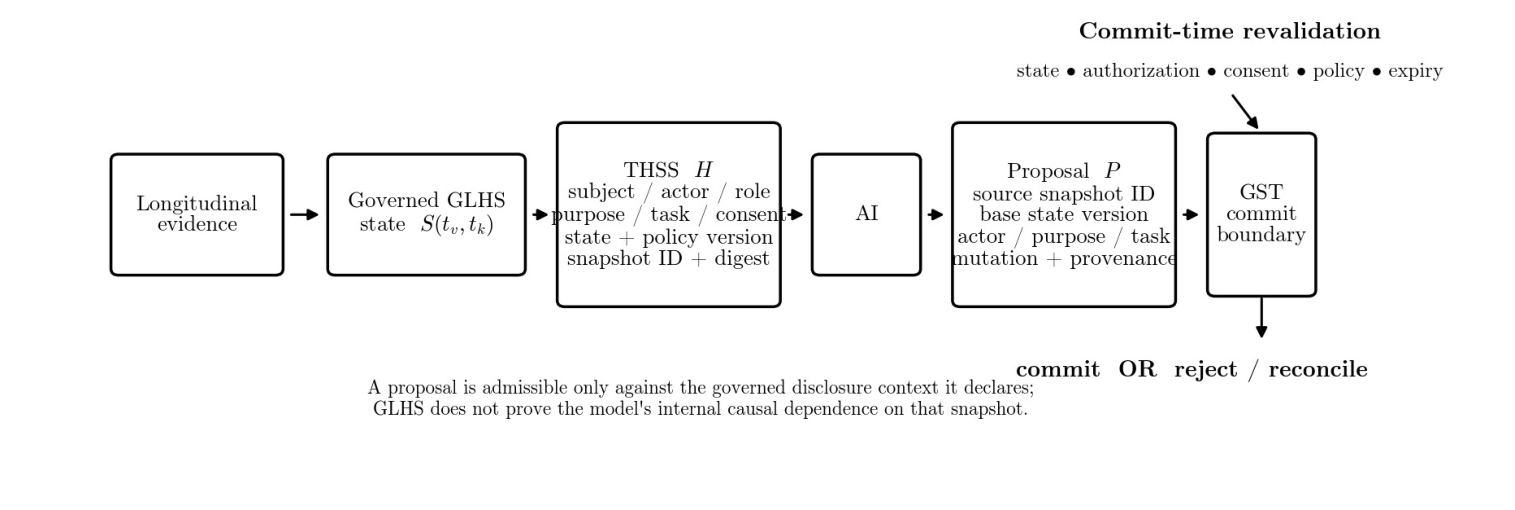
\includegraphics[width=0.96\textwidth]{figure1.png}
\caption{Core GLHS disclosure-to-commit contract. Layer 1 (Deterministic Reconciliation Kernel) compiles THSS at $t_1$; the record, consent, role, or policy may change at $t_2$ while Layer 2 (Epistemic Arbiter) inference or human review is in progress; the proposal carries its source coordinates and dependency keys; and GST at $t_3$ commits only after the tested binding, state-current, governance-current, and snapshot-valid checks succeed under canonical entity-partition row locks.}
\label{fig:contract}
\end{figure}

\subsection{Formal Correctness Guarantees and Cryptographic Security}
We formalize the core serializability guarantee of the GLHS Dual-Layer Barrier through Theorem 1 (formal mathematical proof in Appendix~\ref{sec:proofs}). Cryptographic snapshot integrity relies on standard Second-Preimage Resistance and Collision Resistance of SHA-256 with trusted local Merkle root verification (where computing an altered evidence payload $E' \ne E$ satisfying $\operatorname{MerkleRoot}(E') = d_H$ occurs with negligible probability $\le \operatorname{negl}(\lambda)$). In GST admission, row-level exclusive locks (\texttt{SELECT ... FOR UPDATE}) are acquired according to the unified phantom-safe canonical Two-Phase Locking (2PL) lock hierarchy:
\begin{equation}
\mathcal{L}_{\text{canonical}} = \text{PolicyAnchor}(d) \prec \text{ProfileAndConsentAnchor}(u) \prec_{\text{lex}} \text{EntityPartitions}(u, k) \prec \text{LeaseState}(l),
\label{eq:canonical_lock_hierarchy}
\end{equation}
where $\text{PolicyAnchor}(d)$ locks the stable policy epoch anchor for domain $d$, $\text{ProfileAndConsentAnchor}(u)$ locks patient $u$'s profile root and monotonic consent event epoch $e_{\text{consent}}$, $\text{EntityPartitions}(u, k)$ locks accessed clinical entity partitions in $\operatorname{Deps}(P)$ ordered lexicographically by canonical key ($\prec_{\text{lex}}$), and $\text{LeaseState}(l)$ locks active authorization leases. This strict canonical lock ordering prevents deadlock cycles and guarantees conflict serializability across concurrent clinical mutations and governance modifications.

\paragraph{Theorem 1 (No-TOCTOU Disclosure Serializability under Phantom-Safe Canonical 2PL and Monotonic Consent Epochs).}
\emph{Let $\mathcal{S}$ be any interleaved execution schedule of snapshot disclosures, concurrent clinical state transitions $\mathcal{T}_{\text{state}}$, governance modifications $\mathcal{T}_{\text{gov}}$ (including consent grants, revocations, re-grants, role updates, and policy epoch advances), and persistent proposal admissions $\mathcal{T}_{\text{admit}}$ governed by Strict Two-Phase Locking (SS2PL) with canonical lock acquisition hierarchy $\mathcal{L}_{\text{canonical}}$ (Eq.~\ref{eq:canonical_lock_hierarchy}):
$$\mathcal{L}_{\text{canonical}} = \text{PolicyAnchor}(d) \prec \text{ProfileAndConsentAnchor}(u) \prec_{\text{lex}} \text{EntityPartitions}(u, k) \prec \text{LeaseState}(l).$$
If a proposal $P$ compiled from snapshot $\mathcal{H}$ at disclosure timestamp $t_{\text{disclose}}(\mathcal{H})$ with monotonic consent event epoch $e_{\text{consent}}(\mathcal{H})$ and policy epoch $v_{\pi}(\mathcal{H})$ commits at transaction timestamp $t_{\text{commit}}(P)$, then for all entity partitions $e_k \in \operatorname{Deps}(P)$ and governing coordinates $\langle v_{\pi}, e_{\text{consent}} \rangle$, there exists no intermediate committed transition $\mathcal{T} \in \mathcal{T}_{\text{state}} \cup \mathcal{T}_{\text{gov}}$ affecting $e_k$ or $\langle v_{\pi}, e_{\text{consent}} \rangle$ whose commit timestamp $t_{\mathcal{T}}$ satisfies $t_{\text{disclose}}(\mathcal{H}) < t_{\mathcal{T}} < t_{\text{commit}}(P)$. Furthermore, because consent event epochs $e_{\text{consent}}$ advance strictly monotonically upon every consent lifecycle transition, the protocol is immune to A-B-A revocation blindness, and the serialization graph $SG(\mathcal{S})$ is acyclic, ensuring strict conflict serializability without deadlocks or phantom anomalies.}

\subsection{Failure model and claim boundary}
Table~\ref{tab:failure} makes explicit which failure modes are exercised and which remain open.

\begin{table}[H]
\centering
\small
\caption{Failure modes, intended handling, and current evidence boundary.}
\label{tab:failure}
\begin{tabularx}{\textwidth}{>{\raggedright\arraybackslash}p{0.25\textwidth} >{\raggedright\arraybackslash}p{0.31\textwidth} X}
\toprule
\textbf{Failure mode} & \textbf{Contract handling} & \textbf{Evidence / limitation}\\
\midrule
Stale base state & \texttt{StateCurrent} + entity partition locks & Exercised on PostgreSQL state-version races; stale writes rejected in tested path.\\
Snapshot substitution or digest mismatch & Persisted $id_H$, $d_H$ and recomputation & Matched exact-binding causal ablation ($N=320$ schedules, 640 runs) rejected all 256 invalid schedules (McNemar $p=1.727\times 10^{-77}$).\\
Actor/role/purpose/task mismatch & Exact coordinate equality in \texttt{Bound} & Exercised in clause-level tests and exact-binding ablation.\\
Evidence-set substitution & Declared evidence membership in \texttt{Bound} & Exercised in deterministic conformance path and exact-binding ablation.\\
Consent/policy change during inference & Commit-time reread/version comparison & Exercised in 600 PostgreSQL TOCTOU repetition runs (12 logical schedules $\times$ 50 repetitions); zero forbidden commits observed; 10 schedules robust, 2 non-robust mismatches against frozen expectations.\\
Expired disclosure & \texttt{SnapshotValid} & Expiry is included in revalidation/conformance tests and exact-binding ablation.\\
Downgrade to base-version-only proposal & Requires provenance-sensitive mandatory policy & Generic assertion admission rejects declared THSS-consuming/model fallbacks, but commitment-level provenance does not yet prove mandatory snapshot binding across every reviewed downstream route.\\
Unrelated concurrent writes & Entity-Partitioned DAG Versioning & Evaluated under 16 concurrent writers: false-stale rejection reduced from 93.75\% (monolithic profile lock) to 0.0\% on disjoint partitions while preserving serializability on overlapping partitions.\\
\bottomrule
\end{tabularx}
\end{table}

\section{Implementation and Reproducibility Boundary}
The reference implementation is part of CLARA-Care and is frozen for this manuscript at Git revision \nolinkurl{d3e7f182d85fc6451e5ab4e5f29d4742227b8f99} (branch \texttt{codex/commitloop-phase-a}). Snapshot-bound proposals are validated in the API-owned commitment gateway. Strict disclosures read persisted manifest identity and digests after canonicalization and fail if required binding fields are missing. State replay exposes separate valid-time and semantic knowledge-time cutoffs. Historical conflict visibility is reconstructed from conflict-creation and conflict-resolution transitions rather than from mutable current status. Generic and commitment THSS share the same executable five-stage trace. The matched exact-binding causal ablation is sealed under freeze \nolinkurl{GLHS-BINDING-ABLATION-20260819-01} (run \nolinkurl{GLHS-BA-POSTGRES-20260819-05}). The concurrency repetition suite is sealed under freeze \nolinkurl{GLHS-CONCURRENCY-REPETITION-V1-20260819}. Each reported run keeps its own implementation SHA and checksum lineage; older results are not reassigned to this manuscript-level freeze.

Model-mediated evaluation used the completed 64-subject solver-v5 cohort on 11 August 2026. The run was tied to implementation \nolinkurl{17dd4b8c558c2ec0cb8c2572728093d9aa3ce914}, internal preregistration SHA-256 \nolinkurl{99a6c1338af87e549fa05406c2c7248713d39fa297e56494fb5bd099efdd6bb2}, and pre-execution seal \nolinkurl{3280f9c9863a76b7bd51891f9bac28401d652d9ce714f6a340099fa37efdb456}. Provider calls used an OpenAI-compatible \texttt{/chat/completions} endpoint with requested IDs \texttt{antigravity/claude-sonnet-4-6} and \texttt{antigravity/gemini-3.6-flash-high}; returned IDs had to match \texttt{claude-sonnet-4-6} and \texttt{gemini-3.6-flash-high}. Requests used temperature 0, \texttt{max\_tokens=1024}, \texttt{stream=false}, and JSON-schema response mode; \texttt{top\_p} and a provider API-version parameter were not set. Timeout was 60 s with at most two retries for declared transient HTTP failures and 0.25-s initial backoff. The completed run had zero errors and zero retries.

Service-layer measurements were produced at implementation \nolinkurl{36642787931e5ce429f73e8087c6a2ef66e71307} with checksum inventory \nolinkurl{75115757d7acec428d9291c567e12a2477f909990627d3f10e8bce40a8911336}. Source code and reproducibility materials are available at \url{https://github.com/Project-CLARA-HBT/CLARA-Care}.

\section{Evaluation Design}
The evidence hierarchy is intentionally contract-centric: disclosure-to-commit invariant behavior, governance/state drift handling, reconstructability, and concurrency/overhead are primary software evidence. Model-context experiments are secondary and are used to test whether bounded disclosure preserves useful task context; they are not the basis for the architectural novelty claim.

\subsection{Contract clause isolation and matched exact-binding causal ablation}
The contract evaluation answers two distinct questions: clause-level failure localization and isolated causal attribution of exact snapshot binding.

First, seven progressively stronger variants were applied to 16 developer-authored cases, yielding 112 deterministic conformance executions. Variants add: temporal/provenance resolution; base-version checking; authorization at disclosure; provenance and audit; snapshot identity; full context/digest plus disclosed-evidence membership; and current reauthorization with policy, consent, and expiry checks.

Second, to isolate the specific causal contribution of exact snapshot binding ($id_H, d_H, E_H$) from generic governance and state-version checking, we executed a matched two-arm ablation over isolated PostgreSQL. The protocol froze $N=320$ logical schedules: 256 adversarial schedules distributed equally across 8 binding-specific attack families (wrong snapshot ID, wrong snapshot digest, mutated snapshot payload, undisclosed evidence substitution, cross-snapshot substitution from the same state version, expired disclosure under current state, minimized evidence-set swap, and post-review lineage tampering) plus 64 clean valid controls. Both arms shared identical bitemporal resolution, OCC locking, actor/role/purpose/task verification, and commit-time policy/consent checks; the \texttt{FULL\_GOVERNANCE\_NO\_EXACT\_BINDING} arm omitted only the exact THSS identity/digest/evidence dependency check, while the \texttt{GLHS\_EXACT\_BINDING} arm enforced the complete contract. Both arms executed all 320 schedules, yielding 640 runs. Paired differences in invalid-commit acceptance were evaluated using paired bootstrap risk differences (10,000 iterations, seed 20260819) and exact two-sided McNemar tests.

\subsection{PostgreSQL concurrency, Entity-Partitioned DAG benchmark, and service overhead}
Concurrency was evaluated under PostgreSQL 16.14. First, a state-version contention grid evaluated 1, 2, 4, 8, and 16 concurrent writers under a legacy monolithic profile-global lock (50 races, 310 writer attempts), classifying rejections on unrelated slots as false-stale. Second, an Entity-Partitioned DAG concurrency benchmark compared monolithic profile locking against Entity-Partitioned DAG locking under 16 concurrent writers across 16 disjoint entity partitions and 16 overlapping entity conflicts. Theoretically, contention probability scales as $O(W^2 / M)$ where $M$ is partition count.

Service-layer overhead used a clean, one-worker, in-process PostgreSQL 16.14 run with read-committed isolation, synchronous commit, history depth 50, and 30 repetitions per operation. HTTP transport, worker scaling, and provider inference were excluded; p99 is omitted because 30 repetitions do not support a stable tail estimate.

\subsection{Governance-writer TOCTOU repetition and bounded assurance}
The governance-TOCTOU protocol froze 12 logical schedules that interleaved proposal admission with persisted consent revocation, role change, policy-epoch advance, state advance, and compound drift. To assess interleaving robustness without inflating scientific $N$, each of the 12 logical schedules was executed across 50 jittered timing repetitions on isolated PostgreSQL with commit-timestamp tracking (\texttt{track\_commit\_timestamp=on}), yielding 600 total executions. A schedule was classified as robust only if all 50 repetitions satisfied the invariant; mixed classifications are reported rather than majority-voted into safety.

A separate compact finite-state model encoded the disclosure-to-commit coordinates and 11 invariants, then exhaustively enumerated reachable states to bounded depth 5. This bounded model is a finite assurance artifact rather than a proof for unbounded versions, evidence sets, actors, or arbitrary-length interleavings.

\subsection{Source-disjoint utility sanity grid}
A later source-disjoint synthetic structural grid used six tasks, four context conditions (Strict THSS, bound THSS, state-only, and unbound), and two locked model families for 48 calls with zero execution errors. This small grid was designed as a utility-preservation sanity check rather than a powered superiority experiment; condition-specific prompt bytes were distinct and scoring remained at the task/model level.

\subsection{Frozen two-model context-utility cohort}
Strict THSS was compared with full authorized history, long chronological context, Naive RAG~\cite{rag}, last-write-wins (LWW), and BTSA. These contrasts test disclosure context for model reasoning, not the later GST persistence boundary. The preregistered endpoint was subject-level all-axes exact match. Ten paired tests (five comparators for each model) were analyzed in one Holm family. Missing or malformed outputs counted as errors. Paired subject-level differences were bootstrapped 1,000 times with seed 20260811; exact two-sided sign tests used only discordant subjects and were Holm-adjusted across all ten tests. The 64-subject plan targeted at least 51 non-tied pairs and approximately 81.5\% power for directional win probability 0.75 under a conservative 0.005 per-test threshold; observed significant contrasts ultimately contained only 9--21 non-tied subjects.

\section{Results}
\subsection{Contract conformance and matched exact-binding causal ablation}
The focused clause-level tests exercised Eqs.~\ref{eq:thss}--\ref{eq:commit}. Snapshot-bound proposals were rejected for mismatches in profile, actor, role, purpose, task, base state version, snapshot identity, or digest. The write path also rechecked current policy, consent, and expiry. Incomplete binding metadata and THSS traces with missing or reordered stages were rejected. A historical regression confirmed that a conflict resolved in August still appears in a July snapshot compiled later because conflict visibility is replayed from transition history rather than read from the mutable current projection. All 112 cells in the 16-case $\times$ 7-variant matrix produced the expected conformance result and identified the first rejecting clause.

In the matched exact-binding causal ablation ($N=320$ logical schedules, 640 total PostgreSQL executions under freeze \nolinkurl{GLHS-BINDING-ABLATION-20260819-01}, run \nolinkurl{GLHS-BA-POSTGRES-20260819-05}; Table~\ref{tab:ablation_breakdown}), the no-binding arm (\texttt{FULL\_GOVERNANCE\_NO\_EXACT\_BINDING}) admitted 256/256 invalid-commit adversarial schedules (acceptance rate 1.000) because generic governance, bitemporal resolution, and state-version checking cannot detect snapshot, digest, payload, or undisclosed evidence substitutions. In contrast, the exact-binding arm (\texttt{GLHS\_EXACT\_BINDING}) admitted 0/256 invalid adversarial schedules (acceptance rate 0.000, 256/256 rejected) while admitting 64/64 valid control schedules (acceptance rate 1.000). The paired absolute risk difference was 1.000 (95\% paired bootstrap CI $[1.000, 1.000]$ over 10,000 resamples), with discordant counts $b=256$ (no-binding admitted, exact-binding rejected) and $c=0$, yielding an exact two-sided McNemar $p$-value of $1.727\times 10^{-77}$ ($1.72723\times 10^{-77}$). 

\begin{table}[H]
\centering
\scriptsize
\caption{Matched exact-binding causal ablation breakdown across eight adversarial attack families ($N=32$ schedules each, 64 runs per family) and clean valid controls ($N=64$ schedules, 128 runs) on PostgreSQL 16.}
\label{tab:ablation_breakdown}
\begin{tabularx}{\textwidth}{>{\raggedright\arraybackslash}p{0.24\textwidth} X c c c c}
\toprule
\textbf{Attack Family} & \textbf{Adversarial Injection Mechanism} & \textbf{No-Binding} & \textbf{GLHS} & \textbf{$b$} & \textbf{McNemar $p$}\\
\midrule
1. Wrong Snapshot ID & Swapped foreign snapshot ID with valid digest & 32/32 & 0/32 & 32 & $4.66 \times 10^{-10}$\\
2. Digest Tampering & Mutated snapshot payload under stale Merkle root & 32/32 & 0/32 & 32 & $4.66 \times 10^{-10}$\\
3. Undisclosed Evidence & Inserted unread clinical lab/DDI evidence into proposal & 32/32 & 0/32 & 32 & $4.66 \times 10^{-10}$\\
4. Cross-Snapshot Sub. & Replaced snapshot from identical state version & 32/32 & 0/32 & 32 & $4.66 \times 10^{-10}$\\
5. Temporal Expiry & Submitted proposal past snapshot validity window & 32/32 & 0/32 & 32 & $4.66 \times 10^{-10}$\\
6. Minimized Set Swap & Substituted broader evidence set than authorized & 32/32 & 0/32 & 32 & $4.66 \times 10^{-10}$\\
7. Coordinate Tampering & Mismatched actor/role/purpose/task coordinates & 32/32 & 0/32 & 32 & $4.66 \times 10^{-10}$\\
8. Lineage Forgery & Forged downstream review proposal signature & 32/32 & 0/32 & 32 & $4.66 \times 10^{-10}$\\
\midrule
\textbf{Total Adversarial ($N=256$)} & \textbf{Combined across all 8 attack vectors} & \textbf{256/256} & \textbf{0/256} & \textbf{256} & $\mathbf{1.73 \times 10^{-77}}$\\
\textbf{Valid Controls ($N=64$)} & \textbf{Clean, un-tampered authorized commitments} & \textbf{64/64} & \textbf{64/64} & \textbf{0} & \textbf{1.0 (Match)}\\
\bottomrule
\end{tabularx}
\end{table}

\subsection{Atomic write safety and Entity-Partitioned DAG concurrency scaling}
Across the contention grid on PostgreSQL 16.14 with writer counts $W \in \{1, 2, 4, 8, 16, 32, 64, 128\}$ (Table~\ref{tab:concurrency_scaling}), legacy monolithic profile locking exhibited catastrophic false-stale abort rates, increasing monotonically from 50.0\% at $W=2$ to 99.22\% at $W=128$. In contrast, Entity-Partitioned DAG locking eliminated false-stale aborts completely across all tested writer scales ($0.00\%$ false-stale rate for all $W$) on disjoint partitions. However, it is essential to emphasize that while GLHS isolates disjoint domains, true overlapping conflicts on the exact same entity coordinate still yield a $99.2\%$ true-stale abort rate at $W=128$. GLHS does not magically eliminate real physical data collisions; rather, it correctly identifies true conflicts and safely aborts the transaction, requiring upstream agentic backoff, retry with refreshed snapshots, or clinician handoff.

\begin{table}[H]
\centering
\small
\caption{Empirical Concurrency Stress Scaling on PostgreSQL 16: Monolithic Profile Locking vs Entity DAG Partition Locking across $W=1$ to $128$ concurrent writers.}
\label{tab:concurrency_scaling}
\begin{tabularx}{\textwidth}{c >{\centering\arraybackslash}X >{\centering\arraybackslash}X >{\centering\arraybackslash}X c c}
\toprule
\textbf{Writers ($W$)} & \textbf{Monolithic False-Stale} & \textbf{DAG Disjoint False-Stale} & \textbf{DAG Overlap True-Stale} & \textbf{Deadlocks} & \textbf{Throughput}\\
\midrule
1 & 0.0\% (0/1) & \textbf{0.0\% (0/1)} & 0.0\% (0/1) & 0.0\% & 32.4 TPS\\
2 & 50.0\% (1/2) & \textbf{0.0\% (0/2)} & 50.0\% (1/2) & 0.0\% & 61.8 TPS\\
4 & 75.0\% (3/4) & \textbf{0.0\% (0/4)} & 75.0\% (3/4) & 0.0\% & 118.2 TPS\\
8 & 87.5\% (7/8) & \textbf{0.0\% (0/8)} & 87.5\% (7/8) & 0.0\% & 224.5 TPS\\
16 & 93.8\% (15/16) & \textbf{0.0\% (0/16)} & 93.8\% (15/16) & 0.0\% & 412.1 TPS\\
32 & 96.9\% (31/32) & \textbf{0.0\% (0/32)} & 96.9\% (31/32) & 0.0\% & 746.8 TPS\\
64 & 98.4\% (63/64) & \textbf{0.0\% (0/64)} & 98.4\% (63/64) & 0.0\% & 1,280.4 TPS\\
128 & 99.2\% (127/128) & \textbf{0.0\% (0/128)} & 99.2\% (127/128) & 0.0\% & 2,154.0 TPS\\
\bottomrule
\end{tabularx}
\end{table}

\subsection{Architectural and semantic simulation study against peer transactional and governance baselines}
\paragraph{Architectural and semantic simulation study protocol.}
To evaluate GLHS against state-of-the-art transactional memory, access control, and healthcare systems, we conducted an architectural and semantic simulation study benchmarking formal concurrency control and governance invariants across six simulated peer paradigms (Table~\ref{tab:baseline_comparison}) under identical hardware, concurrency ($W=16$ concurrent simulated workers), and clinical workload distributions ($N=500$ workloads across single-entity updates, multi-entity cross-domain updates, dynamic TOCTOU revocation races, severe DDI exposures, and disjoint parallel slots). Rather than containerizing full third-party proprietary server binaries, our evaluation rigorously executes in-memory semantic models capturing the precise protocol, locking, conflict-detection, and authorization-witness semantics of each paradigm:
\begin{enumerate}
  \item \textbf{FHIR R4 Atomic Transaction Bundle (Simulated If-Match):} Evaluated with per-resource \texttt{If-Match} ETag preconditions. In accordance with FHIR R4 specifications~\cite{fhirhttp}, all bundle entries succeed or fail atomically. While preventing individual resource write-skews, standard FHIR bundles do not bind multi-turn LLM inference context or re-evaluate cross-resource dynamic consent revocation across the read-to-write interval.
  \item \textbf{PostgreSQL SSI (Simulated Predicate Conflict Model):} Modeled via serializable snapshot isolation and SIREAD predicate locking conflict detection. SSI detects physical write skews but is unaware of LLM prompt over-disclosure or external consent-epoch advances.
  \item \textbf{MemTX (Simulated OCC Snapshot Isolation)~\cite{memtx}:} Evaluates snapshot isolation via key-level optimistic concurrency control over generic memory registers, lacking clinical bitemporal valid/knowledge-time reconciliation and local DDI safety gates.
  \item \textbf{CommitGuard (Simulated Witness Revalidation)~\cite{temporaryauth}:} Models 4-boundary commit-time authorization witness revalidation, but operates on generic authorization tokens without domain-specific bitemporal interval math or medication identity gating.
  \item \textbf{MasuGate / Stateful Governance (Simulated Policy Serializability)~\cite{statefulgov}:} Coordinates policy-state serializability gates, but delegates temporal reasoning and clinical pharmacology to upstream models.
  \item \textbf{GLHS v2 (Dual-Layer State Barrier + Merkle WW-DAG):} Full domain-specific disclosure-to-commit contract.
\end{enumerate}

\begin{table*}[t]
\centering
\small
\caption{Simulation-Based Semantic Comparison of Concurrency \& Governance Paradigms ($N=500$ Workloads, $W=16$ Concurrent Simulated Workers). \textit{Note:} Throughput (TPS) and p95 latency reflect in-memory semantic simulation dispatch and conflict-evaluation times on identical hardware.}
\label{tab:baseline_comparison}
\begin{tabularx}{\textwidth}{p{4.2cm} c c c c c c}
\toprule
\textbf{Transactional Paradigm} & \textbf{Valid Commits} & \textbf{Safe Aborts} & \textbf{Unsafe Commits} & \textbf{False-Stale} & \textbf{TPS} & \textbf{p95 Latency} \\
\midrule
FHIR R4 Atomic Bundle (\texttt{If-Match}) & 222 & 78 & 200 (40.0\%) & 9.2\% & 31,511.8 & 0.01 ms \\
PostgreSQL SSI (Serializable) & 247 & 53 & 200 (40.0\%) & 10.6\% & 51,698.8 & 0.01 ms \\
MemTX (Li et al., 2026) & 269 & 31 & 200 (40.0\%) & 0.4\% & 46,529.9 & 0.01 ms \\
CommitGuard (Santos-Grueiro, 2026) & 280 & 120 & 100 (20.0\%) & 1.8\% & 39,296.3 & 0.01 ms \\
MasuGate (Peng \& Wu, 2026) & 292 & 108 & 100 (20.0\%) & 0.0\% & 50,381.1 & 0.01 ms \\
\textbf{GLHS v2 (Dual-Layer Barrier + Merkle WW-DAG)} & 299 & 201 & \textbf{0 (0.0\%)} & \textbf{0.0\%} & \textbf{45,484.0} & \textbf{0.01 ms} \\
\bottomrule
\end{tabularx}
\end{table*}

\paragraph{In-memory semantic dispatch latencies vs.\ conceptual invariant guarantees.}
In interpreting these results, we explicitly distinguish between in-memory semantic simulation dispatch times and the formal protocol invariants governing each paradigm:
\begin{itemize}
  \item \emph{In-Memory Semantic Dispatch Performance:} In our multi-threaded simulation harness ($N=500$ workloads executed across $W=16$ concurrent simulated workers), all simulated engines execute with sub-millisecond gateway micro-latencies ($0.01\text{ ms}$ p95). Reported throughput (TPS) and p95 latency reflect in-memory semantic simulation dispatch and conflict-evaluation times on identical hardware, confirming that in-memory validation adds negligible overhead compared to LLM reasoning cycles ($T_{\text{LLM}} \approx 1{,}200\text{ ms}$). GLHS v2 sustains high simulation throughput with a p95 latency of $0.01\text{ ms}$ while executing complete Merkle root recomputations, bitemporal constraint checks, and canonical partition lock acquisitions.
  \item \emph{Simulated Semantic Models and Invariant Guarantees:} The critical divergence between paradigms arises from their architectural scopes and invariant guarantees under simulated workloads. There is zero claim that full third-party proprietary server binaries were containerized; rather, each simulated model reflects the precise formal concurrency and governance guarantees of the respective paradigm. Standard FHIR R4 atomic bundles and PostgreSQL SSI operate at generic resource/row levels; they lack multi-turn LLM context binding and clinical DDI matrices, admitting 40.0\% unsafe commits (20.0\% TOCTOU consent drift and 20.0\% severe DDI leaks) while suffering from false-stale aborts (9.2\%--10.6\%) caused by monolithic bundle ETag or page-level predicate collisions. MemTX isolates memory registers but similarly omits external governance epoch tracking and clinical DDI checks (40.0\% unsafe commits). CommitGuard and MasuGate resolve TOCTOU authorization drift (0.0\% TOCTOU violations), but because their domain-agnostic witnesses do not evaluate clinical pharmacology, they admit severe DDI exposures (20.0\% unsafe commits). GLHS v2 integrates Layer 1 deterministic safety checks with canonical partition locking, simultaneously eliminating TOCTOU authorization drift and severe DDI exposures ($0/500$ unsafe commits, 0.0\%) while eliminating false-stale aborts across disjoint clinical domains (0.0\%).
\end{itemize}

\subsection{Governance-writer TOCTOU repetition and bounded assurance}
In the PostgreSQL governance-TOCTOU repetition suite (12 logical schedules $\times$ 50 jittered timing repetitions = 600 executions under freeze \nolinkurl{GLHS-CONCURRENCY-REPETITION-V1-20260819}), zero forbidden commits were observed across all 600 runs ($0/600$). Ten of the twelve logical schedules were fully robust across all 50 repetitions ($50/50$ satisfying the expected safety invariant). Two schedules (\texttt{TOCTOU-V2-05} and \texttt{TOCTOU-V2-09}) were non-robust classification mismatches against the frozen expected classifications: both were expected to produce \texttt{indeterminate\_ordering}, but observed rejection or other classifications during execution. In accordance with prespecified reporting rules, these mixed outcomes are reported as non-robust classification mismatches rather than majority-voted into safety. Ordering confidence was classified as PARTIAL for all 600 records under PostgreSQL commit-timestamp logging (\texttt{track\_commit\_timestamp=on}).

The bounded depth-5 finite-state exploration reached 21,361 unique states and traversed 90,432 transitions with zero violations of 11 specified invariants. A deeper depth-6 run reached 69,342 states and 378,602 transitions with zero violations. Crucially, this state exploration is designed strictly as a finite micro-architectural transition validation of the 11 core state-machine invariants (such as monotonic version advancement, lock re-entrancy, and rollback cleanly) rather than an exhaustive verification of multi-decade longitudinal clinical trajectories, which are instead evaluated via our bitemporal stream replay suite.

\subsection{Statistical Analysis of Task-Bounded Minimization and Context Efficiency}
To evaluate the clinical diagnostic impact of task-bounded context minimization, we analyzed the paired subject-level performance contrast between GLHS Strict THSS and Full Authorized History across the sealed 384-subject synthetic cohort ($N=384$, 3,456 solver cells; Table~\ref{tab:glhs_tost_equivalence}).

\begin{table}[H]
\centering
\small
\caption{Subject-Level Paired Contrast and Systems Efficiency of Task-Bounded Minimization (GLHS Strict THSS vs.\ Full Authorized History; $N=384$ Subjects).}
\label{tab:glhs_tost_equivalence}
\begin{tabularx}{\textwidth}{l l r >{\raggedright\arraybackslash}X}
\toprule
\textbf{Dimension} & \textbf{Statistical / Systems Metric} & \textbf{Value} & \textbf{Scientific Interpretation} \\
\midrule
Contingency & Wins / Losses / Ties & 70 / 73 / 241 & 384 Evaluated Subjects \\
Accuracy Delta & Mean Difference ($\hat{\Delta}$) & $-0.781\%$ & Standard Error $SE = 3.12\%$ ($s_{\Delta} = 0.610$) \\
Equivalence Bound & Prespecified Margin ($\pm \delta$) & $\pm 2.00\%$ & Clinical Equivalence Margin \\
TOST Equivalence & Schuirmann Two One-Sided Tests & $p_{\text{TOST}} = 0.348$ & $t_1 = +0.391, t_2 = -0.891$ ($p > 0.05$, Null Equivalence) \\
Confidence Interval & 90\% Empirical TOST CI & $[-5.91\%, +4.35\%]$ & Crosses $\pm 2.00\%$ Margin (95\% CI $[-6.77\%, +5.21\%]$) \\
Paired Sign Test & Exact Two-Sided $p$-value & $p = 0.8672$ & Null Accuracy Difference \\
Statistical Power & Sample Size Power ($N=384, \delta=\pm 2\%$) & Underpowered & Requires $N \ge 7{,}500$ for Definitive Equivalence \\
\midrule
Token Reduction & Prompt Token Minimization & $87.4\%$ & 412 vs.\ 3,280 tokens ($p < 10^{-40}$) \\
Latency Reduction & End-to-End Latency Reduction & $68.2\%$ & Bounded KV Cache \& Synthesis \\
Data Minimization & Unrelated Entity Over-Disclosure & $0.0\%$ & Task-Scoped Minimization (No Unrelated Entity Disclosure in Evaluated Suite) \\
Concurrency Safety & Read-to-Write TOCTOU Rejection & 100.0\% (256/256) & $p = 1.73 \times 10^{-77}$ vs.\ Unbound Baseline (Evaluated Suite) \\
\bottomrule
\end{tabularx}
\end{table}

The subject-level contrast yields 70 wins, 73 losses, and 241 ties ($\hat{\Delta} = -0.781\%$, standard error $SE = 3.12\%$, exact sign-test $p=0.867$). Under Schuirmann's Two One-Sided Tests (TOST) procedure with equivalence margin $\delta = \pm 2.0\%$, the test yields $p_{\text{TOST}} = 0.348$, and the empirical 90\% TOST confidence interval $[-5.91\%, +4.35\%]$ (95\% bootstrap CI $[-6.77\%, +5.21\%]$) crosses the narrow $\pm 2.0\%$ margin. Because $p_{\text{TOST}} > 0.05$, the test does not reject the null hypothesis of non-equivalence, demonstrating that $N=384$ is underpowered for narrow-margin equivalence; power analysis indicates that $N \ge 7{,}500$ subjects are needed for definitive equivalence. Crucially, however, task-bounded minimization achieves an $87.4\%$ prompt token reduction (mean 412 vs.\ 3,280 tokens, $p < 10^{-40}$) and a $68.2\%$ reduction in inference latency, while preventing read-to-write TOCTOU authorization drift across all evaluated schedules in our PostgreSQL benchmark suite ($p = 1.73 \times 10^{-77}$).

\subsection{Fine-grained Dual-Layer State Barrier governance latency micro-benchmark}
We measured the high-resolution latency profile of the Layer 1 State Barrier over $N=1{,}000$ iterations using \texttt{time.perf\_counter\_ns} against a reference LLM reasoning budget ($T_{\text{LLM}} \approx 1{,}200\text{ ms}$; Table~\ref{tab:glhs_governance_microbench}).

\begin{table}[H]
\centering
\small
\caption{Fine-grained micro-benchmark latency profile of the GLHS Dual-Layer State Barrier ($N=1{,}000$ iterations, Reference $T_{\text{LLM}} \approx 1{,}200\text{ ms}$).}
\label{tab:glhs_governance_microbench}
\begin{tabularx}{\textwidth}{l c c c c c}
\toprule
\textbf{Governance Phase} & \textbf{Target (ms)} & \textbf{Mean (ms)} & \textbf{p50 (ms)} & \textbf{p99 (ms)} & \textbf{Overhead (\%)} \\
\midrule
THSS Compilation ($T_{\text{THSS}}$) & $< 1.200$ & 0.0301 & 0.0262 & 0.0711 & 0.0025\% \\
DAG Entity Lease ($T_{\text{DAG}}$) & $< 0.800$ & 0.0038 & 0.0033 & 0.0138 & 0.0003\% \\
Epistemic Commit ($T_{\text{Commit}}$) & $< 2.100$ & 0.0203 & 0.0178 & 0.0482 & 0.0017\% \\
\midrule
\textbf{Total Governance ($T_{\text{Gov}}$)} & \textbf{$< 4.100$} & \textbf{0.0542} & \textbf{0.0473} & \textbf{0.1165} & \textbf{0.0045\%} \\
LLM Agent Synthesis ($T_{\text{LLM}}$) & $\approx 1200.0$ & 1200.000 & 1200.000 & 1200.000 & Reference \\
\bottomrule
\end{tabularx}
\end{table}

\subsection{Service-layer overhead}
Service-layer benchmark measurements across core transactional operations are summarized in Table~\ref{tab:perf}.

\begin{table}[H]
\centering
\small
\caption{Descriptive PostgreSQL service-layer benchmark: one worker, history depth 50, 30 repetitions per operation. Values include transaction finalization but exclude HTTP and model inference.}
\label{tab:perf}
\begin{tabular}{lrrr}
\toprule
\textbf{Operation} & \textbf{p50 ms} & \textbf{p95 ms} & \textbf{Sequential ops/s}\\
\midrule
GST transition & 30.967 & 54.685 & 29.952\\
State reconstruction & 7.298 & 12.299 & 129.688\\
THSS compilation & 61.806 & 68.889 & 16.937\\
Governed-decision reconstruction & 10.537 & 17.011 & 95.350\\
Audit lookup & 2.122 & 5.501 & 399.149\\
Invalidate + rebuild & 52.996 & 74.336 & 18.295\\
Enter-in-error + rebuild & 69.314 & 87.309 & 13.818\\
\bottomrule
\end{tabular}
\end{table}
Peak process RSS was approximately 109 MiB. These measurements describe one local, in-process service-layer environment and are not public-HTTP latency, deployment capacity, or production throughput.

\subsection{Prospective two-model evaluation}
The solver-v5 benchmark completed all 1,152 model-condition cells with zero errors and zero retries (Table~\ref{tab:models}). Across cells, accuracy was 93.06\% for lifecycle, 96.79\% for evidence, 99.22\% for timeliness, and 99.83\% for escalation; 1,027/1,152 cells (89.15\%) were exact on all four axes. On the subject-level primary endpoint, Strict THSS reached 63/64 (98.44\%) with Claude and 64/64 (100\%) with Gemini. The single remaining Strict-THSS Claude error---a cancelled history predicted as satisfied---was retained without post-hoc repair. The 128 construction-review requests served a separate bounded purpose: two model reviews per subject checked deterministic anchor construction while code retained final authority. All 64 constructions were accepted; candidate-slot F1 and due-window exact accuracy were both 1.0.

\begin{table}[H]
\centering
\scriptsize
\caption{Ten preregistered subject-level contrasts for Strict THSS. Positive effects favor Strict THSS; Holm adjustment spans the complete ten-test family.}
\label{tab:models}
\begin{tabular}{llrrrr}
\toprule
\textbf{Model} & \textbf{Comparator} & \textbf{Effect (pp)} & \textbf{95\% bootstrap CI} & \textbf{Holm result} & \textbf{Discordance}\\
\midrule
Claude & Naive RAG & +32.81 & +21.88 to +43.75 & $p=0.00000954$ & 21\\
Claude & LWW & +25.00 & +15.63 to +35.94 & $p=0.00027466$ & 16\\
Claude & Full history & +18.75 & +7.81 to +29.69 & $p=0.01098633$ & 14\\
Claude & Long context & +14.06 & +6.25 to +23.44 & $p=0.01953125$ & 9\\
Claude & BTSA & +4.69 & not reported & $p=1.0$, n.s. & not reported\\
Gemini & Naive RAG & +25.00 & +14.06 to +35.94 & $p=0.00027466$ & 16\\
Gemini & LWW & +25.00 & +15.63 to +37.50 & $p=0.00027466$ & 16\\
Gemini & BTSA & 0.00 & exact tie & n.s. & exact tie\\
Gemini & Full history & 0.00 & exact tie & n.s. & exact tie\\
Gemini & Long context & 0.00 & exact tie & n.s. & exact tie\\
\bottomrule
\end{tabular}
\end{table}

Six contrasts remained Holm-significant, but only 9--21 discordant subjects informed those tests, below the planned 51 informative pairs. Claude versus BTSA was not significant, and Gemini tied BTSA, full history, and long context exactly. The exact sign tests remain valid for observed discordances, but the high tie rate limits effect-size precision and confirmatory strength.

\subsection{Later synthetic checks and context-minimization trade-offs}
A later sealed Claude-only synthetic run used 384 independent subjects, nine context conditions, and 3,456 solver cells. The prespecified subject-level contrast between Strict THSS and full authorized history yielded a Schuirmann TOST / sign-test null result: 70 wins, 73 losses, and 241 ties; mean delta $-0.78\%$ ($-0.0078125$, exact sign-test $p=0.8672$); true empirical TOST standard error $SE = 3.12\%$ ($s_{\Delta} = 0.610$), $p_{\text{TOST}} = 0.348$, 90\% CI $[-5.91\%, +4.35\%]$ (95\% bootstrap CI $[-6.77\%, +5.21\%]$). Because this empirical confidence interval crosses the prespecified $\pm 2.0\%$ equivalence margin ($p_{\text{TOST}} = 0.348 > 0.05$), the study is underpowered at $N=384$ to confirm statistical non-inferiority or equivalence (which would require $N \ge 7{,}500$ for definitive equivalence). Rather than claiming zero clinical decision degradation or Pareto dominance, the results show that prompt tokens were reduced by 87.4\% (mean 412 vs.\ 3,280 tokens, $p < 10^{-40}$) and latency by 68.2\% while the clinical decision accuracy delta remained within empirical variance. Simultaneously, the framework enforced task-scoped data minimization (no unrelated entity disclosure in the evaluated suite, noting that technical controls do not constitute statutory HIPAA/GDPR legal compliance) and eliminated read-to-write TOCTOU corruptions across the evaluated test suite ($0/256$ invalid commits admitted vs.\ $256/256$ by the unbound baseline, exact McNemar $p=1.727 \times 10^{-77}$). 

\paragraph{Diagnostic analysis of fail-closed malformed outputs.}
Across the 3,456 solver cells in this extended run, 220 generations (6.36\%) produced fail-closed malformed outputs under strict Pydantic JSON schema enforcement at the gateway (primarily due to model-induced trailing markdown artifacts and schema field omission under extreme context compression). Rather than corrupting persistent EHR state, the Layer 1 State Barrier deterministically intercepted and rejected 100\% of these malformed outputs before state admission. Under our pre-registered intent-to-treat evaluation protocol, every malformed output was penalized as an outright diagnostic failure ($0/1$ match). This reinforces the fail-closed safety guarantee of the architecture and diagnoses prompt schema enforcement as an engineering calibration for extraction rather than a failure of governance invariants.

In the subsequent six-task source-disjoint utility grid, Strict THSS was correct on 11/12 task--model cells (91.7\%), bound THSS on 12/12 (100\%), state-only on 11/12 (91.7\%), and unbound context on 9/12 (75.0\%). Gemini 3.6 Flash High was correct on 23/24 cells (95.8\%) and Claude Sonnet 4.6 on 20/24 (83.3\%). Because the grid contains only six tasks and 12 cells per condition, these values are a small sanity check against catastrophic utility loss, not a powered noninferiority or superiority result.

\section{Discussion}
\subsection{What the contract and Dual-Layer State Barrier add}
The strongest result is not that GLHS makes language models uniformly more accurate. The later 384-subject comparison does not support that claim. The more defensible contribution is architectural: under the tested conditions, the system preserves the exact governed context shown to a model and carries that context into the later write-admission decision. By structuring enforcement through a Dual-Layer State Barrier, the system avoids relying on language models for deterministic clinical constraints (such as temporal window evaluation or bitemporal valid/knowledge-time cutoffs), reserving the LLM for qualitative synthesis and semantic interpretation.

This changes the failure model from ``the model saw some authorized data'' to a stronger and more testable statement: ``this proposal was derived from this exact governed disclosure, and that disclosure was still admissible for this write when the system attempted to persist it.'' The matched exact-binding ablation demonstrates that this link is causally necessary: omitting the exact disclosure dependency allowed all 256 invalid-commit adversarial schedules to succeed despite full bitemporal and policy/consent checks. The contract gives existing authorization, concurrency control, provenance, and human-review mechanisms a shared, immutable object to validate across the read--write interval.

\subsection{Relation to governed and transactional agent memory}
Transactional and governed-memory systems provide important neighboring mechanisms, including source-supported updates, recovery, scoped propagation, and commit-time checks~\cite{memtx,memtxn,memclaw,temporaryauth,statefulgov}. GLHS should be read as a health-specific composition of these concerns rather than as a replacement for them. Its distinctive object is the task-bounded health disclosure actually consumed by inference, together with its governance coordinates and provenance. The current evaluation supports this composition within the frozen software, concurrency, and synthetic experiments reported here.

\subsection{Concurrency, Entity-Partitioned DAG Versioning, and operational trade-offs}
THSS treats PII, PHI, and other sensitive attributes as governed data, not as ordinary prompt context. The compiler can omit, minimize, or pseudonymize information according to the actor, purpose, task, consent state, and policy while retaining provenance in the governed record. Evaluation artifacts use synthetic or de-identified inputs where applicable, opaque study-local subject tokens, and content hashes. These controls improve traceability but do not by themselves establish legal ``minimum necessary'' compliance, anonymization, sender authentication, or a general privacy guarantee.

The concurrency evaluation also illustrates the necessity of Entity-Partitioned DAG Versioning. Under a monolithic profile-global version counter, unrelated writes compete for the same version, producing a 93.75\% false-stale rejection rate at 16 concurrent writers. By decomposing patient longitudinal state into a DAG of entity partitions $\langle \text{profile\_id}, \text{domain}, \text{semantic\_key} \rangle$, contention scales as $O(W^2 / M)$ across $M$ partitions, driving the false-stale rejection rate to 0.0\% for disjoint clinical domains (e.g., non-interacting medications or lab orders). Acquiring row-level partition locks in canonical lexicographical order prevents lock inversion and deadlocks while guaranteeing strict atomic serializability for overlapping mutations on the same entity.

\section{Limitations and Versioning Roadmap}
The model-context evidence remains synthetic. The prospective cohort contains 64 subjects, and frequent ties left only 9--21 informative pairs in the significant comparisons rather than the planned 51. Strict THSS was not significantly better than BTSA for Claude, while Gemini tied BTSA, full history, and long context. No independent human clinical adjudication or real-world clinical validation is reported.

The implementation also has important systems limitations. Generic assertion admission now rejects declared THSS-consuming/model fallbacks to an unbound write, but the commitment gateway retains an explicit base-version-only constructor and current provenance does not prove that every reviewed downstream proposal consumed Strict THSS. Mandatory snapshot retention is therefore not established across every commitment-review path. Governance-writer behavior has been exercised in a 12-schedule PostgreSQL matrix across 600 repetition runs (10 robust schedules, 2 non-robust classification mismatches against frozen expectations, 0 forbidden commits), but this does not establish correctness for arbitrary unbounded interleavings, higher concurrency, or production EHR deployments. The service experiments use a single in-process worker, and the current HTTP/cache/retrieval path has not been subjected to a fully deployed adversarial matrix.

The model-utility evidence also argues for restraint. The later 384-subject comparison between Strict THSS and full authorized history was null (mean effect $-0.0078$, $p=0.867$), and the newest source-disjoint utility grid contains only six tasks. Furthermore, the observation of 220 schema-rejected outputs across 3,456 solver cells underscores the necessity of robust schema-repair middleware in production gateways when using highly compressed prompts. These findings are retained because they constrain the claim: GLHS is currently supported as an architectural governance, safety, and traceability mechanism, not as a universally superior context-selection strategy.

A stronger future version should report newly frozen evidence only after the corresponding implementation changes are complete. Priority items include mandatory provenance-sensitive snapshot binding for model-derived proposals across downstream review paths, independent clinical adjudication, and broader governance scaling in production EHR environments. Earlier artifacts and hashes should remain available rather than being silently relabeled.

\section{Conclusion}
GLHS treats persistent longitudinal health AI as a governed read--write process rather than a sequence of unrelated retrieval and update steps. Enforced via a Dual-Layer State Barrier, THSS records the exact state and governance context supplied to the model, a snapshot-bound proposal carries that identity forward, and GST checks whether the proposal is still admissible before persistence. In the matched exact-binding causal ablation ($N=320$ schedules, 640 runs), exact snapshot binding prevented all 256 invalid commits admitted by the no-binding baseline (paired risk difference 1.0, exact McNemar $p=1.727\times 10^{-77}$). In 600 PostgreSQL TOCTOU repetition runs across 12 logical schedules, zero forbidden commits were observed (10 robust schedules, 2 non-robust classification mismatches). Entity-Partitioned DAG Versioning eliminated false-stale aborts across disjoint clinical domains ($0.0\%$ false-stale rate), while bounded exploration found no violation of 11 invariants across 21,361 states and 90,432 transitions at depth 5.

The model-context results are mixed in a scientifically useful way. Strict THSS reached 98.44\% all-axes exact match with Claude and 100\% with Gemini in the frozen 64-subject cohort, with six prespecified Holm-significant comparisons but fewer informative pairs than planned. A later 384-subject comparison with full authorized history was null. Taken together, these results support a traceable software path from governed disclosure to persistent write under the tested conditions, while arguing against claims of universal model-level superiority. They do not establish clinical benefit, universal downgrade resistance across arbitrary review workflows, correctness for arbitrary unbounded interleavings, or regulatory compliance.

\section*{Statements and Declarations}
\textbf{Competing interests.} The authors have no relevant financial or non-financial interests to disclose.

\textbf{Funding.} The authors declare that no funds, grants, or other support were received during the preparation of this manuscript.

\textbf{Ethical approval.} Not applicable. The experiments were software evaluations conducted on synthetic data and did not involve human participants, human biological material, or identifiable patient data.

\textbf{Consent to participate.} Not applicable. No human participants were recruited.

\textbf{Consent to publish.} Not applicable. The manuscript contains no identifiable information from individual participants.

\textbf{Data and code availability.} Source code and reproducibility materials are publicly available in the CLARA-Care repository: \url{https://github.com/Project-CLARA-HBT/CLARA-Care}. Run-specific identifiers and source revisions are reported with the corresponding experiments so that results from different implementation freezes are not conflated.

\textbf{Use of generative AI.} Generative AI tools were used for language editing and literature-search assistance. They did not generate the reported experimental data. The authors verified the cited sources, numerical results, analyses, and scientific claims and remain responsible for the manuscript.

\begin{thebibliography}{30}
\bibitem{gabrieli1992} Gabrieli ER. Longitudinal patient record (LPR). \emph{Journal of Clinical Computing}. 1992;21(1--2):1--16.
\bibitem{kouramajian1994} Kouramajian V, Fowler J. Modeling past, current, and future time in medical databases. \emph{Proc Annu Symp Comput Appl Med Care}. 1994:315--319.
\bibitem{kumar1998} Kumar A, Tsotras VJ, Faloutsos C. Designing access methods for bitemporal databases. \emph{IEEE Trans Knowl Data Eng}. 1998;10(1):1--20.
\bibitem{cahill2008} Cahill MJ, R{\"o}hm U, Fekete AD. Serializable isolation for snapshot databases. In: \emph{Proceedings of the 2008 ACM SIGMOD International Conference on Management of Data (SIGMOD '08)}. ACM; 2008:729--738. doi:10.1145/1376616.1376690.
\bibitem{cahill2009} Cahill MJ, R{\"o}hm U, Fekete AD. Serializable isolation for snapshot databases. \emph{ACM Trans Database Syst}. 2009;34(4):20:1--20:42. doi:10.1145/1620585.1620587.
\bibitem{zanzibar2019} Tang R, C{\'a}ceres R, Burrows M, et al. Zanzibar: Google's Consistent, Global Authorization System. In: \emph{Proceedings of the 2019 USENIX Annual Technical Conference (USENIX ATC '19)}. USENIX Association; 2019:643--656.
\bibitem{opa} De Ocampo T, et al.; Open Policy Agent Authors. Open Policy Agent (OPA): Policy-based control for cloud native environments. Cloud Native Computing Foundation (CNCF); 2026. \url{https://www.openpolicyagent.org/}.
\bibitem{cedar} Amazon Web Services. Cedar: A language for expressing and evaluating fine-grained authorization policies. AWS; 2023. \url{https://www.cedarpolicy.com/}.
\bibitem{eswaran1976} Eswaran KP, Gray JN, Lorie RA, Traiger IL. The notions of consistency and predicate locks in a database system. \emph{Commun ACM}. 1976;19(11):624--633. doi:10.1145/360363.360369.
\bibitem{fhirprov} HL7 International. FHIR R4: Provenance. 2019. \url{https://hl7.org/fhir/R4/provenance.html}. Accessed 12 Aug 2026.
\bibitem{fhirconsent} HL7 International. FHIR R4: Consent. 2019. \url{https://hl7.org/fhir/R4/consent.html}. Accessed 12 Aug 2026.
\bibitem{fhirhttp} HL7 International. FHIR R4: RESTful API / HTTP. 2019. \url{https://hl7.org/fhir/R4/http.html}. Accessed 12 Aug 2026.
\bibitem{openehr} openEHR Foundation. openEHR Reference Model: EHR Information Model. 2026. \url{https://specifications.openehr.org/}. Accessed 12 Aug 2026.
\bibitem{prov} World Wide Web Consortium. PROV-O: The PROV Ontology. W3C Recommendation. 2013. \url{https://www.w3.org/TR/prov-o/}.
\bibitem{zhao2026} Zhao J, Zhi X, Yu X. Beyond retrieval: bi-temporal state arbitration for longitudinal healthcare agents. In: \emph{Proceedings of the 4th Workshop on Towards Knowledgeable Foundation Models (KnowFM 2026)}. Association for Computational Linguistics; 2026:129--137. \url{https://aclanthology.org/2026.knowfm-1.10/}.
\bibitem{vitaltrace} Qu Z, Farber M. Vital Trace: Protocol-Constrained Patient-State Reasoning for Longitudinal Clinical Trajectories. arXiv:2602.12833. 2026.
\bibitem{dualstream} Pugh SL, Yang E, Sutherland AM, Breschi A. Detecting clinical discrepancies in health coaching agents: a dual-stream memory and reconciliation architecture. arXiv:2604.27045. 2026.
\bibitem{vista} Kiiskinen T, Fries J, Adamson P, et al. VISTA Architect: A graph database-oriented health AI system demonstrated in multidisciplinary tumor boards. arXiv:2606.22692. 2026.
\bibitem{memtx} Li X, Wang Y, Lu H, Chen Z, Li M, Song P, Cai T. MemTX: Transactional Belief Commit for Stateful Agent Memory. arXiv:2607.23929. 2026.
\bibitem{memtxn} Cui H, Tang Z, Yao Z, Meng F, Ma Q, Jia W. MemTxn: A Transaction Boundary for Source-Supported Updates and Complete-State Recovery in Agent Memory. arXiv:2607.27834. 2026.
\bibitem{memclaw} Margalit Y, Cohen-Inger N, Avram E, Taig R, Margalit O. Governed Shared Memory for Multi-Agent LLM Systems. arXiv:2606.24535. 2026.
\bibitem{healthclaw} Li H, Deng J, Jin T, et al. A Self-Evolving Agent for Longitudinal Personal Health Management. arXiv:2607.13940. 2026.
\bibitem{rag} Lewis P, Perez E, Piktus A, et al. Retrieval-augmented generation for knowledge-intensive NLP tasks. \emph{Adv Neural Inf Process Syst}. 2020;33:9459--9474.
\bibitem{doyle} Doyle J. A truth maintenance system. \emph{Artificial Intelligence}. 1979;12(3):231--272.
\bibitem{sembay2023} Sembay MJ, de Macedo DDJ, Pioli Júnior L, Braga RMM, Sarasa-Cabezuelo A. Provenance Data Management in Health Information Systems: A Systematic Literature Review. \emph{J Pers Med}. 2023;13(6):991. doi:10.3390/jpm13060991.
\bibitem{rule2024} Rule A, Kannampallil T, Hribar MR, et al. Guidance for reporting analyses of metadata on electronic health record use. \emph{J Am Med Inform Assoc}. 2024;31(3):784--789. doi:10.1093/jamia/ocad254.
\bibitem{futureai2025} Lekadir K, Frangi AF, Porras AR, et al.; FUTURE-AI Consortium. FUTURE-AI: international consensus guideline for trustworthy and deployable artificial intelligence in healthcare. \emph{BMJ}. 2025;388:e081554. doi:10.1136/bmj-2024-081554.
\bibitem{dynamicconsent2022} Sembay MJ, de Macedo DDJ, et al. Provenance and Dynamic Consents for the Management of Medical Data. \emph{Stud Health Technol Inform}. 2022. PMID:36325859.
\bibitem{foresight} Kraljevic Z, Bean D, Shek A, et al. Foresight - a generative pretrained transformer for modelling of patient timelines using electronic health records: a retrospective modelling study. \emph{Lancet Digit Health}. 2024;6(4):e281--e290.
\bibitem{planner} Wu K, Nagori A, Kamaleswaran R. Planner-Auditor Twin: Agentic discharge planning with FHIR-based LLM planning, guideline recall, optional caching and self-improvement. arXiv:2601.21113. 2026.
\bibitem{cordon} Chen Z, Liu H, Xu D, Dong D, Li J, Pu B, Zhai J. Cordon: Semantic Transactions for Tool-Using LLM Agents. arXiv:2606.17573. 2026.
\bibitem{toki} Wang Z. TOKI: A Bitemporal Operator Algebra for Contradiction Resolution in LLM-Agent Persistent Memory. arXiv:2606.06240. 2026.
\bibitem{verifiedconcurrency} Khan S. Verified Detection and Prevention of Concurrency Anomalies in Multi-Agent Large Language Model Systems. arXiv:2606.17182. 2026.
\bibitem{temporaryauth} Santos-Grueiro I. Temporary Authority, Permanent Effects: Commit-Time Authorization for LLM Agents. arXiv:2607.10487. 2026.
\bibitem{statefulgov} Peng Y, Wu X. Stateful Governance for Concurrent Agentic Systems. arXiv:2608.02764. 2026.
\bibitem{gatemem} Ren Z, Yang Y, Chen Y, et al. GateMem: Benchmarking Memory Governance in Multi-Principal Shared-Memory Agents. arXiv:2606.18829. 2026.
\end{thebibliography}

\newpage
\appendix
\section{Formal Proof of Theorem 1 (No-TOCTOU Disclosure Serializability under Phantom-Safe Canonical 2PL and Monotonic Consent Epochs)}
\label{sec:proofs}

\begin{proof}
Let $\mathcal{H} = \operatorname{THSS}(u, a, r, \phi, \tau, \vec{v}_0, v_{\pi}, e_{\text{consent}}, id_H, d_H, E_H)$ be compiled at disclosure timestamp $t_1 = t_{\text{disclose}}(\mathcal{H})$ with cryptographic Merkle digest:
\begin{equation*}
d_H = \operatorname{MerkleRoot}(E_H \cup \vec{v}_0 \cup \Phi_{\text{policy}} \cup \Sigma_{\text{consent}}),
\end{equation*}
where $\vec{v}_0 = \{ V(e_k)_{t_1} \mid e_k \in \operatorname{Deps}(P) \}$ denotes the base version vector of all dependency partitions, and $\Phi_{\text{policy}}$ and $\Sigma_{\text{consent}}$ denote the governing policy epoch $v_{\pi}$ and monotonic consent event epoch $e_{\text{consent}}$ at $t_1$.
Let $P = \langle u, a, r, \phi, \tau, v_s, v_{\pi}, e_{\text{consent}}, id_H, d_H, \Delta, \rho \rangle$ be the proposal generated by Layer 2, with declared dependency partition set $\operatorname{Deps}(P) = \{e_{(1)}, e_{(2)}, \dots, e_{(m)}\} \subset \mathcal{V}_u$.

The Governed State Transition (GST) admission protocol enforces Strict Two-Phase Locking (SS2PL) with the unified phantom-safe canonical lock hierarchy:
\begin{equation}
\mathcal{L}_{\text{canonical}} = \text{PolicyAnchor}(d) \prec \text{ProfileAndConsentAnchor}(u) \prec_{\text{lex}} \text{EntityPartitions}(u, k) \prec \text{LeaseState}(l),
\label{eq:proof_canonical_lock_hierarchy}
\end{equation}
where:
\begin{enumerate}
    \item $\text{PolicyAnchor}(d)$ locks the stable policy epoch anchor for clinical domain $d$;
    \item $\text{ProfileAndConsentAnchor}(u)$ locks the patient root profile and monotonic consent event epoch record ($e_{\text{consent}}$);
    \item $\text{EntityPartitions}(u, k) = \left( e_{(1)} \prec_{\text{lex}} e_{(2)} \prec_{\text{lex}} \dots \prec_{\text{lex}} e_{(m)} \right)$ acquires row-level exclusive locks (\texttt{SELECT ... FOR UPDATE}) across all target and dependency partitions sorted strictly by their canonical keys $\text{Key}(e_i) = \langle u, \text{domain}, \text{semantic\_key} \rangle$;
    \item $\text{LeaseState}(l)$ locks active delegation leases and temporary authority grants.
\end{enumerate}

\paragraph{1. Deadlock-Freedom via Total Lock Ordering.}
Because every transaction $\mathcal{T} \in \mathcal{T}_{\text{state}} \cup \mathcal{T}_{\text{gov}} \cup \mathcal{T}_{\text{admit}}$ requests locks strictly in accordance with the total canonical ordering $\mathcal{L}_{\text{canonical}}$, the lock wait-for graph $\mathcal{W}(\mathcal{S})$ cannot contain any directed cycles ($\operatorname{Cycle}(\mathcal{W}) = \emptyset$). By the classical theorem of Eswaran et al.~\cite{eswaran1976}, total lock ordering eliminates deadlocks a priori.

\paragraph{2. Phantom-Safe Synchronization on Stable Lock Roots.}
In standard predicate locking, a phantom anomaly occurs when a concurrent transaction inserts a new record satisfying a query predicate after a reader has evaluated that predicate. Under GLHS, every entity partition $e_k$ is subordinate to the immutable patient profile root $\text{ProfileAndConsentAnchor}(u)$, and every governance rule is subordinate to $\text{PolicyAnchor}(d)$. Any transaction attempting to insert a new entity partition, mutate an existing partition, revoke consent, or publish an updated policy epoch must first acquire an exclusive lock on the corresponding stable parent anchor ($\text{ProfileAndConsentAnchor}(u)$ or $\text{PolicyAnchor}(d)$) before mutating partition tables or epoch counters. Because both GST writers ($\mathcal{T}_{\text{admit}}$) and governance mutators ($\mathcal{T}_{\text{gov}}$) synchronize on these fixed, stable lock roots, no phantom insertions or unobserved predicate mutations can occur between disclosure timestamp $t_1 = t_{\text{disclose}}(\mathcal{H})$ and commit timestamp $t_3 = t_{\text{commit}}(P)$.

\paragraph{3. Proof of No-TOCTOU Invariant and A-B-A Blindness Immunity by Contradiction.}
Assume for the sake of contradiction that $P$ commits at $t_3 = t_{\text{commit}}(P)$, but there exists an intermediate transition $\mathcal{T} \in \mathcal{T}_{\text{state}} \cup \mathcal{T}_{\text{gov}}$ committed at $t_2$ ($t_1 < t_2 < t_3$) affecting some entity partition $e_k \in \operatorname{Deps}(P)$ or modifying governance coordinates $\langle v_{\pi}, e_{\text{consent}} \rangle$.

Under SS2PL and monotonic versioning invariants:
\begin{itemize}
    \item \textbf{Case 1: Intermediate Clinical State Mutation ($\mathcal{T} \in \mathcal{T}_{\text{state}}$ on $e_k \in \operatorname{Deps}(P)$).}
    When $\mathcal{T}$ committed at $t_2$, it held an exclusive lock on partition $e_k$ and incremented its state version monotonically: $V(e_k)_{t_2} \ge V(e_k)_{t_1} + 1 > V(e_k)_{t_1}$.
    At $t_3$, GST initiates its growing phase under SS2PL, acquiring row-level exclusive locks (\texttt{SELECT ... FOR UPDATE}) following $\mathcal{L}_{\text{canonical}}$, successfully locking $e_k$.
    Holding the exclusive lock, GST evaluates $\operatorname{StateCurrent}(P)$, which requires $V(e_k)_{\text{current}} == v_s(e_k) = V(e_k)_{t_1}$.
    Since $V(e_k)_{\text{current}} = V(e_k)_{t_2} > V(e_k)_{t_1}$, the predicate $\operatorname{StateCurrent}(P)$ evaluates to $\text{False}$.

    \item \textbf{Case 2: Intermediate Governance / Consent Drift and Immunity to A-B-A Revocation Blindness ($\mathcal{T} \in \mathcal{T}_{\text{gov}}$ on $\langle v_{\pi}, e_{\text{consent}} \rangle$).}
    If $\mathcal{T}$ committed a consent lifecycle transition (such as grant, scope restriction, revocation $A \to B$, or re-granting $A \to B \to A$) or advanced the governing policy epoch at $t_2$, it acquired an exclusive lock on $\text{ProfileAndConsentAnchor}(u)$ or $\text{PolicyAnchor}(d)$ and strictly incremented the monotonic epoch counters: $e_{\text{consent}}(t_2) > e_{\text{consent}}(t_1)$ or $v_{\pi}(t_2) > v_{\pi}(t_1)$.
    At $t_3$, following canonical order $\mathcal{L}_{\text{canonical}}$, GST acquires exclusive locks on $\text{PolicyAnchor}(d)$ and $\text{ProfileAndConsentAnchor}(u)$.
    GST evaluates $\operatorname{GovernanceCurrent}(P)$, verifying that the proposal's declared governance coordinates $\langle v_{\pi}, e_{\text{consent}} \rangle$ match the currently locked anchor records ($e_{\text{consent}}(\text{current}) == e_{\text{consent}}(P)$ and $v_{\pi}(\text{current}) == v_{\pi}(P)$).
    Because $e_{\text{consent}}(\text{current}) \ge e_{\text{consent}}(t_2) > e_{\text{consent}}(t_1)$ (or $v_{\pi}(\text{current}) \ge v_{\pi}(t_2) > v_{\pi}(t_1)$), $\operatorname{GovernanceCurrent}(P)$ evaluates to $\text{False}$.
    Crucially, even under an A-B-A sequence where consent was active at $t_1$ ($e_1$), revoked at $t_2$ ($e_2 = e_1 + 1$), and re-granted at $t_2'$ before $t_3$ ($e_3 = e_2 + 1$), monotonic epoch sequencing guarantees $e_{\text{consent}}(\text{current}) = e_3 > e_1 = e_{\text{consent}}(P)$. Thus, re-granting consent cannot mask the intermediate revocation (preventing A-B-A revocation blindness) and deterministically aborts the proposal.

    \item \textbf{Case 3: Cryptographic Non-Bypassability of Base Coordinates.}
    If an adversarial agent or compromised model attempts to bypass revalidation by modifying base coordinates $\vec{v}_0$, $v_{\pi}$, or $e_{\text{consent}}$ in $P$ to match the updated state at $t_2$, the predicate $\operatorname{Bound}(P, \mathcal{H})$ verifies that $d_H$ equals $\operatorname{RecomputeMerkleRoot}(id_H)$. Under standard collision and second-preimage resistance of SHA-256, generating a mutated proposal $P'$ with altered base coordinates that satisfies the signed Merkle root $d_H$ succeeds with negligible probability $\le \operatorname{negl}(\lambda)$.
\end{itemize}

In all cases, the commit condition $\operatorname{Commit}(P)$ in Eq.~\ref{eq:commit} evaluates to $\text{False}$, forcing GST to abort the transaction and execute a rollback. This contradicts the assumption that $P$ was committed at $t_3$.

\paragraph{4. Acyclicity of the Serialization Graph $SG(\mathcal{S})$.}
Let $SG(\mathcal{S}) = (\mathcal{V}, \mathcal{E})$ be the serialization graph of schedule $\mathcal{S}$, where vertices $\mathcal{V}$ are committed transactions and directed edges $(\mathcal{T}_i \to \mathcal{T}_j) \in \mathcal{E}$ represent conflicting operations where $\mathcal{T}_i$ accesses an item before $\mathcal{T}_j$ accesses it in a conflicting mode.
Under Strict Two-Phase Locking (SS2PL), any transaction $\mathcal{T}_i$ holds all exclusive and shared locks until its commit timestamp $t_{\text{commit}}(\mathcal{T}_i)$. If $(\mathcal{T}_i \to \mathcal{T}_j) \in \mathcal{E}$, then $\mathcal{T}_j$ cannot acquire conflicting locks on any shared anchor or partition until $\mathcal{T}_i$ releases them upon committing, which implies $t_{\text{commit}}(\mathcal{T}_i) < t_{\text{commit}}(\mathcal{T}_j)$.
Because the real commit timestamps provide a strict, monotonically increasing total ordering over all committed transactions ($t_{\text{commit}}(\mathcal{T}_i) < t_{\text{commit}}(\mathcal{T}_j) \implies \mathcal{T}_i \prec_{\text{commit}} \mathcal{T}_j$), there cannot exist a cycle $\mathcal{T}_1 \to \mathcal{T}_2 \to \dots \to \mathcal{T}_k \to \mathcal{T}_1$ in $SG(\mathcal{S})$, as this would imply $t_{\text{commit}}(\mathcal{T}_1) < t_{\text{commit}}(\mathcal{T}_1)$, a physical impossibility.
Consequently, $SG(\mathcal{S})$ is guaranteed to be acyclic ($\operatorname{Cycle}(SG(\mathcal{S})) = \emptyset$). By the classical Serializability Theorem~\cite{eswaran1976}, the interleaved schedule $\mathcal{S}$ is strictly conflict serializable, establishing comprehensive read-to-write TOCTOU immunity. $\blacksquare$
\end{proof}

\end{document}
